\documentclass[9pt]{report}
\usepackage[spanish]{babel}
\usepackage[utf8]{inputenc}
\usepackage{graphicx}
\usepackage{caption}
\title{Reconocimiento de Género con Visión por Computadora}
\date{Julio de 2021}
\author{Julio Ponce C. y Angel Maldonado G.}
\usepackage{vmargin}
\usepackage{multicol}
\setmargins{1.73cm}
{1.9cm}
{18.1356cm}
{23.495cm}
{10pt}
{1cm}
{0pt}
{2cm}

\newenvironment{Figura}
  {\par\medskip\noindent\minipage{\linewidth}}
  {\endminipage\par\medskip}

\begin{document}
	\begin{center}
		{\scshape\huge Reconocimiento de Género por Visión Artificial\par}
		\vspace{0.5cm}
		{\large Julio Ponce Camacho y Angel Maldonado García \par}
		{\large Junio 2022 \par}
		\vspace{0.5cm}
	\end{center}
	
	\begin{multicols}{2}
	\begin{center}
	\section*{Resumen}
	\end{center}
	\paragraph{El reconocimiento del genero de una persona abre las posibilidades de desarollar nuevas herramientas, tanto administrativas (como el control de personas o asignación de espacios/roles) como preventivas (prevención de la violencia de género). El reconocimiento de género dentro de una institución educativa es de vital importancia ya que, como se menciona en el párrafo anterior, la prevención de violencia de género es un tema con grán importancia a día de hoy, sin embargo, el implementarlo en un entorno real resulta complejo, debido al poder computacional requerido en los dispositivos necesarios. Dicho proceso, requiere de entrenamiento en caso de que sea por inteligencia artificial, otorgando un modelo preentrenado para que el dispositivo embebido como los raspberry pi puedan poverlo sin problema.}
	\paragraph{Suponiendo que el software funciona de manera correcta, se podrá aplicar a diferentes puntos de la institución facilitando estadísticas posteriores sobre la violencia de género, permitiendo, en una futura estancia, el poder implementar un sistema de alertas cuando se detecte dicha violencia.}
	\paragraph{Palabras Clave}Detección de Género, Violencia de Género, Inteligencia Artificial, Visión por computadora.
	\begin{center}
	\section*{Introducción}
	\end{center}	
	\paragraph{}
	De acuerdo con el gobierno de México, ha aumentado la conciencia por la violencia de género en el país, a la par de las manifestaciones, 76\% respecto al año anterior \cite{Indice_de_paz}. Sin embargo los homicidios han incrementado en los últimos 5 años, como podemos apreciar en la imagen 1\ref{figura1} se ha aumentado cerca de un 116\%.
	\begin{Figura}
			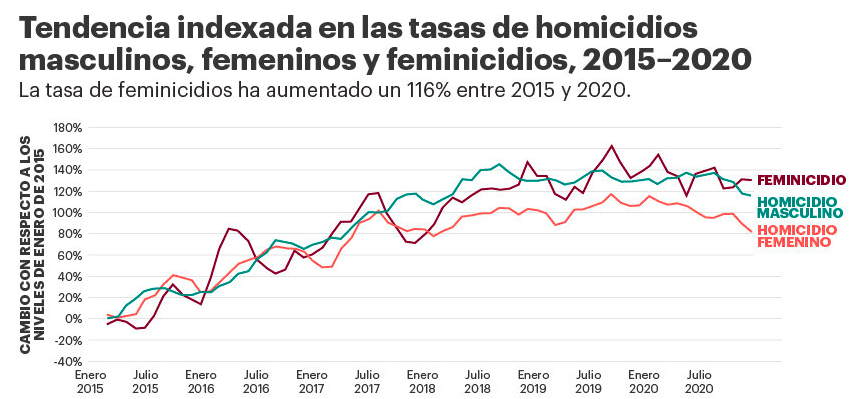
\includegraphics[width=\textwidth]{TendenciasHomicidios2015-2020}
			\captionof{figure}{Tendencia de homicidios en méxico \cite{Indice_de_paz}.}
			\label{figura1}
		\end{Figura}
	\paragraph{}
	Según Casillas, Dorantes y Ortiz, exponen que una de las problemáticas que más aquejan a las universidades de México es la violencia de género que se oculta de manera casi deliverada \cite{CasillasDorantesyOrtiz}.	
	\paragraph{}
	Con base en lo antes mencionado nos enfocamos como un todo, en un sistema de reconocimiento de violencia de género mediante visión por computadora, tomando como punto de partida un software de reconocimiento de género, el cual lo detecte con un video de entrada, tomando cada fotograma de dicho video, recortando cada una de las personas detectadas y decidiendo si se trata de un hombre o una mujer, a la par de detectar un aproximado de su edad. Esto nos ayudará a comenzar con el desarrollo de un istema completo de deteccion de violencia de género, abriendo la posibilidad de implementar el reconocimiento de violencia, que, a la par del reconocimiento de género, podremos obtener métricas interesantes en los entornos en los que se aplique este sistema. Dichas métricas podrían ser: qué genero es el que incurre más en la violencia, en qué edades las personas son más porpensas a ser más violencias y finalmente, en qué entornos las personas son más violentas.
	
	\begin{center}
	\section*{Revisión del estado del Arte}
	\end{center}
	\paragraph{}
	En \cite{GenderDetectionIndia} se propone una solución a la detección de género mediante el uso de bosques de clasificación aleatoria ``Random Forest Classifier'' y Árboles de Decisión de Clasificación ``Decision Tree Classifier''. Las tecnologías usadas son python y el editor de jupyter, la metodología propuesta fue el uso de un dataset de diferentes datos y patrones por los cuales obtuvieron resultados interesantes al momento de reconocer rostros, a partir de esto, se reconocen las edades y los géneros de las personas. Con resultados por encima del 80\% de precisión.
	\paragraph{}
	En \cite{DeepColorization} se habla sobre la colorimetría para la detección de género, para ello utilizaron las librerías incluidas en el framework de aprendizaje profundo ``Caffe'' llamado CNN, el data set que se utilizó fue de 1246 imágenes, para el reconocimiento del genero se utilizó una versión reducida de GoogLeNet incluida igualmente en el framework mencionado, dicho framework permiía hacer la clasificación de las personas mediante capas. Los resultados que obtivieron mejoraban con relación a las iteraciones que se hacian, fando en el peor de los casos un 94\%.
	\paragraph{}
	En \cite{FacialGender} se hace el reconocimiento de género mediante diferentes filtros y algoritmos de clasificación a la par de una estandarización y segmentación de las imagenes, una vez que se obtenía eso, se genera un vector que se usará como template para finalmente aplicarlo a las nuevas immágnes recibidas. Se utilizaron ecuaciones de PCA 
	\begin{center}
		\section*{Metodología}
	\end{center}
	\paragraph{}
	La visión por computadora es aquel campo de estudio que dota a las computadoras la capacidad de identificar imágenes y videos tal como lo haría un ser humano, siendo que la computadora adquiere, procesa y analiza imágenes digítales con el fin de generar información útil para la toma de decisiones sobre algún rubro. En este proyecto de investigación se planteo el desarrollo de un sistema que a través de la visión por computadora sea capaz de identificar rostros, genero y una aproximación de la edad que el sujeto puede tener, con el fin de identificar la posible violencia de genero que puede existir en cierta situación ya que hoy en día lamentablemente ha aumentado rápidamente este tipo de situaciones.
	\paragraph{}
	Para el desarrollo de este software con las capacidades mencionadas previamente, se hizo uso de diversas tecnologías que nos permiten el desarrollo de programas que permiten el procesamiento y análisis de imágenes para la detección de objetos animados e inanimados. En la actualidad uno de los lenguajes de programación más utilizados en la implementación y desarrollo de la inteligencia artificial python, el cual es un lenguaje de alto nivel de programación interpretado, el cual cuenta con gran cantidad de librerías y módulos que permiten prácticamente realizar cualquier cosa en la creación de softwares, desde la creación de programas básicos o la lógica de una página web hasta la creación e implementación de modelos de aprendizaje para la inteligencia artificial en distintos tipos de ámbitos. Por lo tanto, el lenguaje de programación python es el lenguaje base que se utilizó en este proyecto por las diversas características que posee.
	\paragraph{}
	Para el procesamiento de imágenes, una de las tecnologías que se suelen utilizar a menudo es OpenCV abreviado del inglés Open Source Computer Vision, la cual es una biblioteca de código abierto para la visión por computadora y aprendizaje automático con la capacidad de procesar imágenes y videos en tiempo real, al tiempo que cuenta con diversas capacidades analíticas. Una ventaja de esta herramienta es que cuenta con la compatibilidad con distintos marcos de aprendizaje profundo como TensorFlow, Caffe y Pytorch los cuales simplifican en gran medida el proceso de recopilación de datos que luego se pueden usar para el entrenamiento de redes neuronales. Por todo lo mencionado, OpenCV es la tecnología base que se utilizo para la identificación de rostros, edad y genero de las personas.
	\paragraph{}
	Como anteriormente se mencionó, OpenCV hace uso de marcos de aprendizaje profundo, los cuales permiten entrenar la red neuronal para reconocer determinados patrones en imágenes específicas, por lo que para el desarrollo de este proyecto se hicieron uso de modelos pre-entrenados con Caffe, los cuales están diseñados para implementarse en redes neuronales convolucionales, las cuales son ampliamente utilizadas para el reconocimiento y procesamiento de imágenes con base a diversas capas de entrada y salida, que de cierto modo se pueden catalogar como perceptrones multicapa regularizados. Esta elección de este tipo de redes neuronales es gracias a que permiten el reconocimiento sin importar el eje o posición en la que se encuentre el objeto ya que lo puede reconocer gracias a los patrones que este encuentra, a diferencia de una red neuronal normal que solo permite el reconocimiento cuando se es tal cual la imagen y muestra poca precisión cuando existe un pequeño cambio.
	\paragraph{}
	Para la implementación este proyecto, se hizo uso de Deep learning para identificar lo mas preciso posible el genero y edad de una persona a partir de la secuencia de imágenes que un dispositivo de video capte. El genero a reconocer es entre masculino y femenino y la edad se realiza a través de un conjunto de rangos. Los rangos de edad a los que el sujeto identificado puede clasificarse son: (0-2), (4-6), (8-12), (15-20), (25-32), (38-43), (48-53), (60-100), por lo que son 8 nodos en la capa final de Softmax, la cual permite comprimir las salidas de cada neurona para que estas sean 0 y 1 de tal forma que las salidas sea igual a 1 lo que permite realizar una calificación dependiendo si la probabilidad esta entre 0 o 1. La razón por la cual el reconocimiento de edad esta entre esos rangos y no es un valor exacto es debido a que el clasificar una imagen con precisión es bastante difícil debido a la cantidad de factores que pueden influir a la hora de determinar la edad de una persona, como lo son el maquillaje, la iluminación, las obstrucciones y las expresiones fáciles que pueden provocar cambios faciales que pueden dar resultados poco asertivos por parte de la red neuronal, y esto es algo normal incluso en los seres humanos, ya que es muy complicado adivinar la edad de alguien y comúnmente nunca se acierta, por ello es que únicamente se da un aproximado con base a los datos obtenidos.
	\paragraph{}
	La arquitectura de las redes neuronales convolucionales utilizadas para este proyecto en python tienen como característica 3 capas convolucionales. La primera capa convolucional hace uso de 96 nodos y un tamaño del kernel 7, la segunda capa convolucional hace uso de 256 nodos y un tamaño de kernel 5 y la tercera capa hace uso de 384 nodos y un tamaño de kernel 3. Se tienen 2 capas completamente conectadas, cada una con 512 nodos y una capa final de salida de tipo Softmax como se mencionó en el párrafo anterior. Esta arquitectura es la que tienen los modelos utilizados para la implementación del reconocimiento de género y edad.
	\paragraph{}
	Cada uno de los modelos utilizados cuentan con un archivo protobuf (búfer de protocolo), el cual cuenta con el contenido gráfico y los pesos entrenados por el modelo con la extensión “.pb” el cual contiene los valores en formato binario, sin embargo, también se hace uso de archivos “.prototxt” que son el mismo protobuf, pero estos están en formato de texto para hacer uso de ellos, los cuales fueron generados a través de Tensorflow. También se hicieron uso de archivos “.caffemodel” que definen los estados internos de los parámetros de las capas. Cada uno de estos archivos son los que permiten un buen funcionamiento de la red neuronal para la clasificación de los sujetos que la cámara detecte.
	\paragraph{}
	El funcionamiento básico de este sistema se representa en la figura 2, en el cual primero antes de realizar cualquier acción se cargan los archivos protobuf y el modelo en el programa, básicamente se almacena la dirección de su ubicación en alguna variable dentro del programa. Una vez colocada la dirección de los modelos, se crean con base a la dirección de los modelos las redes neuronales, una para el reconocimiento facial, otro para el reconocimiento de género y por último para el reconocimiento de edad. Una vez concretados estas acciones iniciales, se accede al dispositivo de video especificado por el usuario para obtener la secuencia de imágenes a reconocer y seguido de ello se inicia el procesamiento de imágenes. El procesamiento y clasificación de las imágenes lleva la siguiente secuencia:
	\begin{enumerate}
		\item Se realiza la detección de todos los rostros que existan dentro de la imagen obteniendo las coordenadas en las que se encuentra el rostro.
		\item Si se detectaron rostros, continua, si no se detectó ningún rostro regresa a la obtención de imágenes por parte del dispositivo de video.
		\item Se procesa la imagen con base a la red de identificación de género, clasificándolo con base a mujer u hombre.
		\item Se realiza la clasificación de la edad con base al dato más próximo en los rangos establecidos en el modelo.
		\item Si hay mas rostros, vuelve a repetir el proceso desde el reconocimiento de genero (Paso 3) si no es así, continuar.
		\item Dibuja un rectángulo y coloca texto sobre la imagen con los valores identificados.
		\item Vuelve a la captura de video.
	\end{enumerate}
	\paragraph{}
	\begin{Figura}
		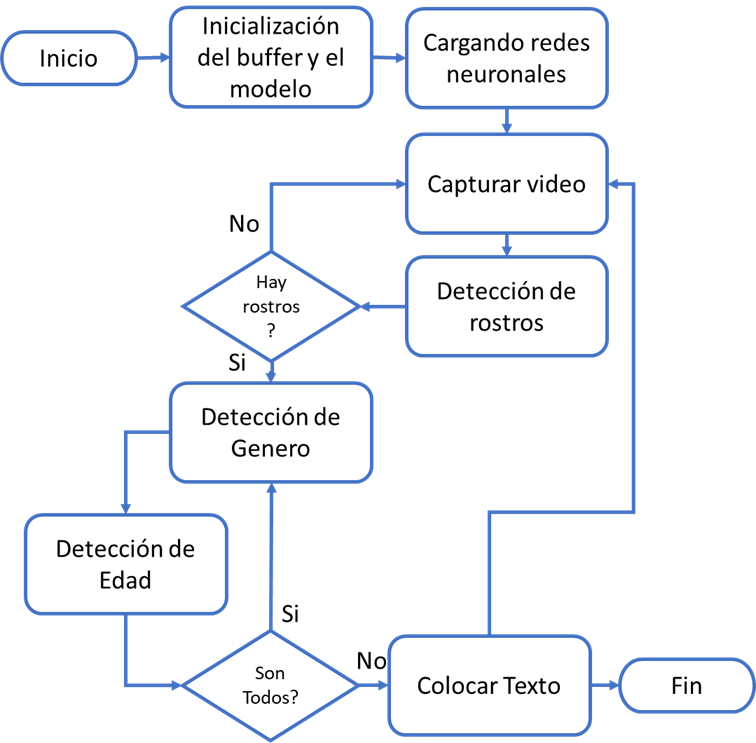
\includegraphics[width=\textwidth]{1}
		\captionof{figure}{Funcionamiento del reconocimiento y clasificación.}
		\label{figura2}
	\end{Figura}
	\paragraph{}
	Este proceso permite realizar el reconocimiento bastante preciso, pero hablando mas sobre esto, el reconocimiento facial toma como parámetros principales los ojos, la nariz y la boca, para determinar si efectivamente lo analizado en la imagen es una persona.
	\begin{Figura}
		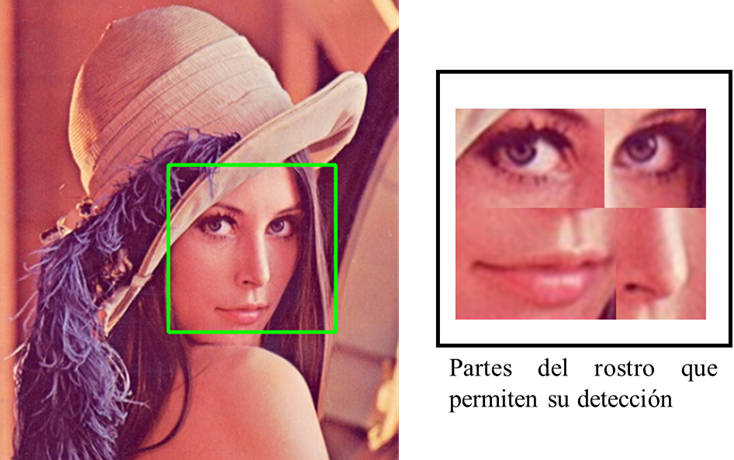
\includegraphics[width=\textwidth]{2}
		\captionof{figure}{Facciones del reconocimiento Facial.}
		\label{figura3}
	\end{Figura}
	\paragraph{}
	Para la identificación de que se hombre o mujer se hacen uso de diversas métricas, como lo es el tamaño de las cejas, las pestañas, el bello facial y el ancho del rostro de la persona. El cabello en este caso no se considera un factor a usar debido a que un hombre o mujer puede tener cabello largo o corto.
	\begin{Figura}
		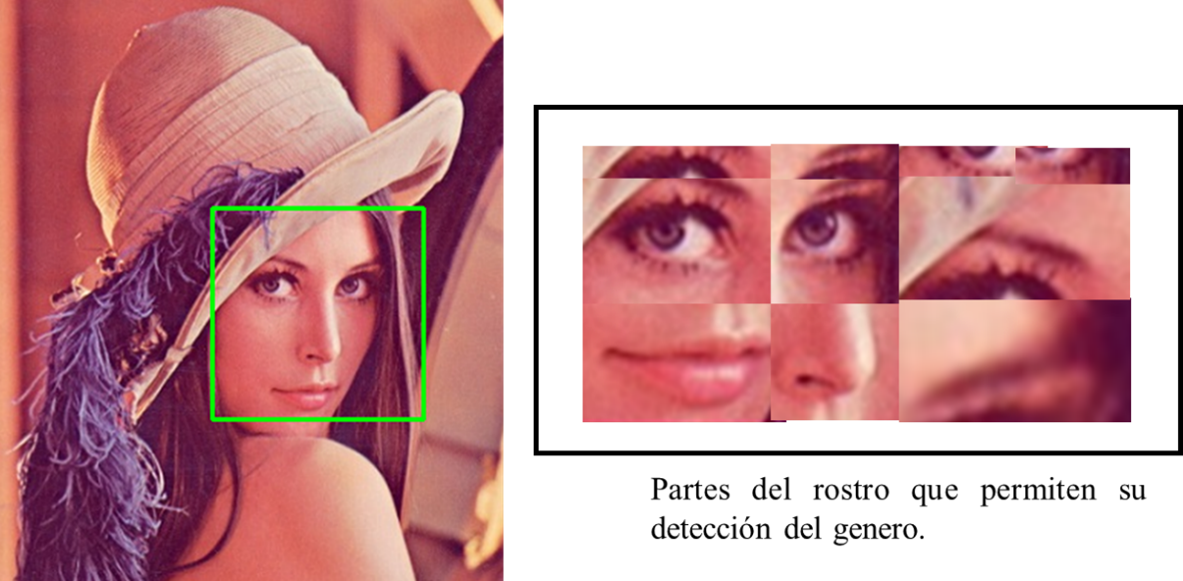
\includegraphics[width=\textwidth]{3}
		\captionof{figure}{Facciones del reconocimiento de Genero.}
		\label{figura4}
	\end{Figura}
	\paragraph{}
	Para la identificación de la edad es algo mas complicado ya que existen múltiples factores que influyen en la edad de una persona y hay aspectos que complican mas aun su reconocimiento como lo son aspectos como el maquillaje o las expresiones faciales, sin embargo, los atributos principales a considerar es el bello facial, el tamaño del rostro, el tamaño de las mejillas y el tamaño de los ojos.
	\paragraph{}
	Para la interfaz de este software, se planteo el uso de las herramientas graficas que python ofrece directamente, sin embargo, estas ofrecían características bastante básicas y daban una apariencia sencilla con el acceso único desde la misma máquina. Para una mejor implementación, y la adición de la característica de poder acceder al sistema de manera remota, se opto por implementar el software como una aplicación Web, a través de HTML, CSS y JavaScript como parte del Frontend y se hizo uso de FLASK como parte del backend, el cual es un framework de python que permite la creación de aplicaciones Web con el uso de pocos recursos con las características necesarias para la conexión entre el frontend y el procesamiento lógico con python.
	\paragraph{}
	La arquitectura de este sistema web se puede ver en la figura 5, en donde primero se establecen los modelos para el reconocimiento con OpenCV y seguido se crea el servidor Flask para que se pueda acceder a la interfaz a través de un navegador Web en maquetado a través del lenguaje de marcado HTML, los estilos CSS y JavaScript. Cuando el usuario accede a la dirección del servidor se muestra la interfaz y en automático se crean respuestas por parte de OpenCV donde se accede al dispositivo de video y se realiza el reconocimiento y clasificación de los rostros, retornando el resultado a FLASK el cual lo manda a un div establecido en el HTML para la visualización del usuario. Dentro de la misma interfaz del usuario se pueden configurar diversos parámetros del video para eficientizar mas el reconocimiento facial, con el fin de optimizar manualmente el brillo o contraste en caso de que se necesario, esto se realiza a través de diversas barras y entradas, las cuales una vez modificadas una función de JavaScript detecta los cambios y guarda sus valores en un objeto JSON, para después mandarlo a través de AJAX al servidor FLASK que lo recibe como diccionario para hacer uso de esos parámetros y configurar los aspectos de la imagen.
	\begin{Figura}
		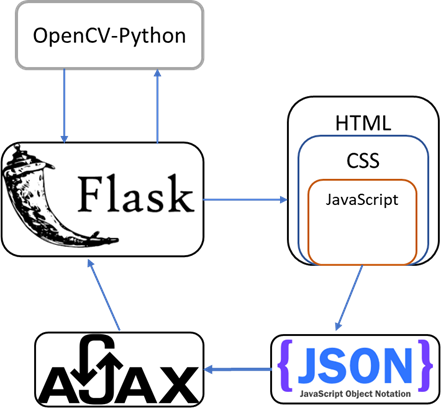
\includegraphics[width=\textwidth]{4}
		\captionof{figure}{Arquitectura del sistema.}
		\label{figura5}
	\end{Figura}
	\paragraph{}
	La interfaz del software desarrollado quedo distribuido de tal forma que, si la pantalla es mayor a 1000 pixeles, el video se mostrara en la parte derecha y los controles para la visualización de la imagen están en la parte derecha, como se puede ver en la figura 6.
	\begin{Figura}
		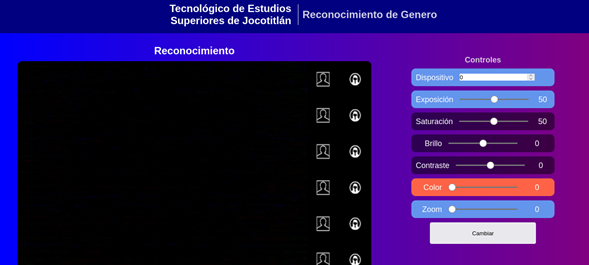
\includegraphics[width=\textwidth]{5}
		\captionof{figure}{Diseño del sistema Web.}
		\label{figura6}
	\end{Figura}
	\paragraph{}
	Al realizar el reconocimiento, si es una persona varón se dibuja un rectángulo azul y se colocan las letras encima colocando si es hombre y la aproximación de edad. Si el rostro reconocido es femenino, el rectángulo a dibujar es color beige y se colocan de igual forma las letras en la parte superior. Estas letras cambian de tamaño dependiendo de la distancia a la que se encuentre la persona que es captada en la cámara.
	\paragraph{}
	La gran ventaja de hacer uso de redes neuronales convolucionales, es que la detección se hace con base a los patrones que coincidan, sin importar si la imagen captada tiene diferencias a comparación las imágenes usadas para el entrenamiento, por ende, este sistema es preciso en el reconocimiento incluso aunque el usuario tenga cubrebocas. 
	\begin{Figura}
		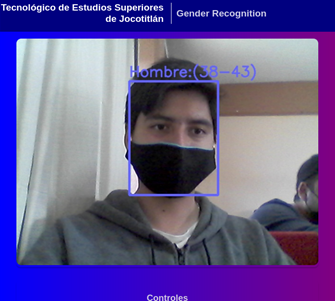
\includegraphics[width=\textwidth]{6}
		\captionof{figure}{Reconocimiento de Genero y Edad.}
		\label{figura7}
	\end{Figura}


	\paragraph{}
	Un aspecto fundamental a la hora de desarrollar cualquier tipo de software de computadora es el uso de recursos que este tenga, ya que todos los sistemas tienen recursos limitados, por lo cual es importante el considerar que es lo que se necesita para que un software pueda funcionar en una computadora.
	\paragraph{}
	En el campo de la inteligencia artificial, se realizan diversos procesos que toman gran parte de los recursos del sistema para poder realizar una acción especifica, y hablando de el reconocimiento facial en tiempo real estos procesos se realizan de manera consecutiva y repetida, por lo cual genera un gran consumo de los recursos, siendo una carga de trabajo bastante grande para el procesador en especial.
	\paragraph{}
	En las pruebas realizadas se hizo uso de una computadora laptop con un procesador APU Ryzen 3 4300u con 8 GB de RAM DDR4. Para la primera prueba no se hizo el reconocimiento de ninguna persona, solo se dejó la cámara sin ningún objetivo para ver cual es el consumo del sistema cuando no existe ningún sujeto, lo cual dio un consumo medio, ya que el procesador se encontraba en un promedio del 49\% de uso, lo cual es relativamente alto considerando que la cámara estaba tapada sin ningún reconocimiento. El uso memoria RAM se mantuvo en 3.2 GB.
	\begin{Figura}
		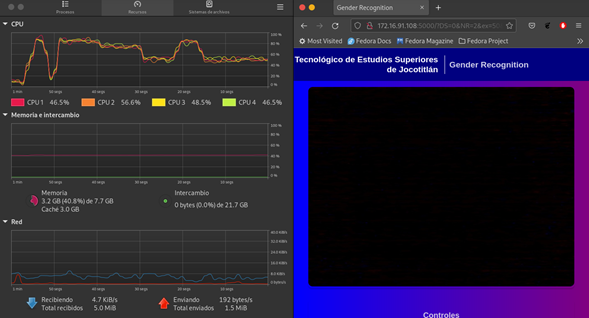
\includegraphics[width=\textwidth]{7}
		\captionof{figure}{Consumo en modo reposo.}
		\label{figura8}
	\end{Figura}
	\paragraph{}
	Para la segunda prueba se hizo el reconocimiento de un rostro, en el cual el consumo aumento un 30\% llegando a ocupar un promedio del 87\% de la capacidad de procesamiento del procesador y el consumo de memoria se mantuvo igual.
	\begin{Figura}
		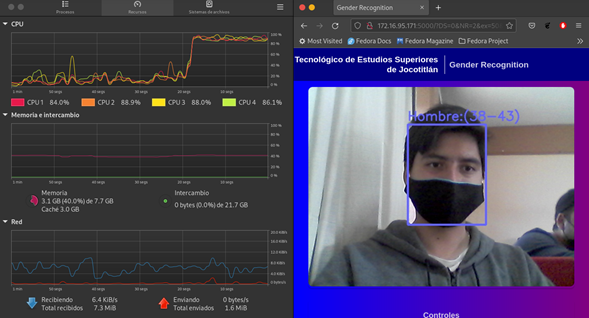
\includegraphics[width=\textwidth]{8}
		\captionof{figure}{Consumo al reconocer una persona.}
		\label{figura9}
	\end{Figura}
	\paragraph{}
	En la siguiente prueba se hizo el reconocimiento de 2 personas, y el procesador aumento un 4\% de uso, siendo que ocupo un promedio del 92\% del procesador.
	\begin{Figura}
		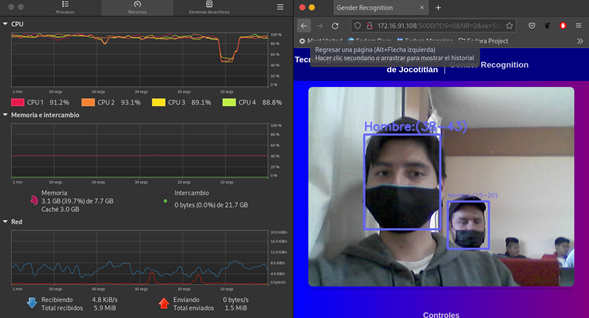
\includegraphics[width=\textwidth]{9}
		\captionof{figure}{Consumo al reconocer dos personas.}
		\label{figura10}
	\end{Figura}
	\paragraph{}
	En la cuarta prueba el numero de sujetos a reconocer aumento a 3, siendo igual de preciso en el reconocimiento de los rostros y el tipo de genero de estos, sin embargo, el consumo aumento otro 3\%, manteniendo el uso del procesador hasta un 94\% de uso y el espacio de memoria se mantuvo igual, por lo que la carga en el procesador era aún mayor.
	\begin{Figura}
		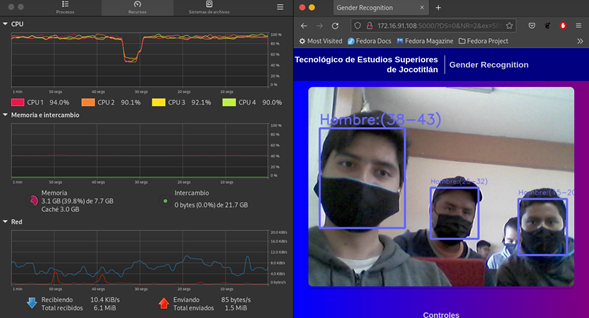
\includegraphics[width=\textwidth]{10}
		\captionof{figure}{Consumo al reconocer tres personas.}
		\label{figura11}
	\end{Figura}
	\paragraph{}
	En la ultima prueba se hizo el reconocimiento de más rostros, en este caso fueron 5 personas, las cuales fueron reconocidas exitosamente, sin embargo, el angular de la cámara estaba algo mas limitado. El uso del aumento 3\% mas que cuando se reconocieron 3 rostros, llegando hasta el 96\% del uso del procesador.
	\begin{Figura}
		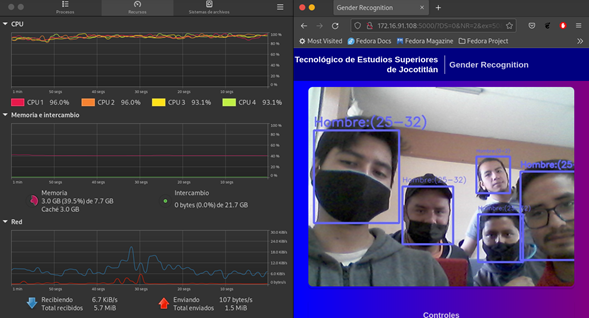
\includegraphics[width=\textwidth]{11}
		\captionof{figure}{Consumo al reconocer cinco personas.}
		\label{figura12}
	\end{Figura}
	\paragraph{}
	Con base a las pruebas se pudo determinar que el reconocimiento facial funciona de manera precisa, así como el reconocimiento de género en la mayoría de los casos es eficaz, sin embargo, el reconocimiento de la edad tiende a ser impreciso en ciertos momentos, dando una edad menor a la que el sujeto pertenece. 
	\paragraph{}
	En temas de rendimiento, el consumo en reposo es bajo comparado a cuando empieza el reconocimiento ya que aumenta hasta un 30\% de uso, sin embargo, por cada rostro que reconoce aumenta alrededor de un 3\% de consumo, por lo cual a partir de 5 personas la carga en el procesador es bastante grande, por lo cual es recomendable hacer uso de un sistema de mayor potencia o bien, utilizar la aceleración por hardware para hacer uso de la tarjeta grafica en el procesamiento de las imágenes,
	\begin{thebibliography}{0}
			\bibitem{Indice_de_paz} IEP México, ``Indice de Paz en México''(2021)[Online], Disponible en: https://www.indicedepazmexico.org/violencia-de-gnero.
			\bibitem{CasillasDorantesyOrtiz} Casillas M., Dorantes J. y Ortiz V., ``Estudios sobre la violencia de en la universidad'', Biblioteca Digital de Humanidades. Universidad Veracruzana (2017).
			\bibitem{GenderDetectionIndia} DR.C.K.Gomathy , Mr.A.Lokesh ,Mr.CH.HARSHAVARDHAN REDDY, Mr.A.SAI KIRAN, ``Age and Gender Detection'' IJSREM, vol. 5, 5pp, Octubre de 2021.
			\bibitem{DeepColorization} J. Hogervorst, E. Okfor y M. Wiering, Institute of Artificial Intelligence and Cognitive Engineering, Faculty of Science and Engineering, University of Groningen, The Netherlands,``Deep Colorization for Facial Gender Recognition'' 9pp, Noviembre de 2017.
			\bibitem{FacialGender} F. Yaghmaee1 y R. Khammari, Journal of Interdisciplinary Studies, ``Facial Gender Recognition, diferent approaches'' , SRPH, 5pp, Diciembre de 2020.			

	\end{thebibliography}	
	\end{multicols}
\end{document}